%%%%%%%% Sample LaTeX input for Complex Systems %%%%%%%%%%% 
% Revision 4, Jun 27, 2018
%
% This is a LaTeX input file  
% Text following % on a particular line is treated as a comment, and 
% ignored by LaTeX.  
% You do not need to type any text that follows a % 
% 
\documentclass{article}

\usepackage{graphicx,hyperref}
\usepackage{amssymb,ComplexSystems}
\usepackage{tikz}
\usepackage{scalefnt}

\usetikzlibrary{automata, positioning, arrows}
\usepackage{underscore}
\graphicspath{ {./images/} }

\usepackage{listings}
\usepackage{color}

\definecolor{dkgreen}{rgb}{0,0.6,0}
\definecolor{gray}{rgb}{0.5,0.5,0.5}
\definecolor{mauve}{rgb}{0.58,0,0.82}

\lstset{frame=tb,
  language=SQL,
  aboveskip=2mm,
  belowskip=3mm,
  showstringspaces=false,
  columns=flexible,
  basicstyle={\small\ttfamily},
  numbers=none,
  numberstyle=\tiny\color{gray},
  keywordstyle=\color{blue},
  commentstyle=\color{dkgreen},
  stringstyle=\color{mauve},
  breaklines=true,
  breakatwhitespace=true,
  tabsize=3
}

% complex-systems.sty is the macro package for Complex Systems.
% It is available at
% http://www.complex-systems.com/samples/complex-systems.sty
% epsf.sty is the preferred graphics import method
\makeindex

\begin{document}
\lstset{language=SQL}
\title{Documentation - Data Bases 2 (Group 21)%
% Use \\ to indicate line breaks in titles longer than about 
% 55 characters. 
%
}

\author{\authname{Marco Fasanella}\\[2pt] 
% Use \\[2pt] to end the line and add space between author name and affiliation. 
\authadd{MsC Computer Science, Polimi}\\
\authadd{C.P. 10617541}\\
\and
% For extra space, precede the second set of authors with \and.
\authname{Nicola Dean}\\
\authadd{MsC Computer Science, Polimi}\\
\authadd{C.P. 10674826}\\
% Do not use a ``.'' at the end of any line in the address. 
}

% The following specifies the running headings 
%
% Each running heading should be less than about 50 characters long. 
% If necessary, give a shortened version of the title. 
%
% Use initials for first and second names. If all author names do not fit, truncate the 
% list and end with ``et al.''.
\markboth{Data Base 2 Project} 
{Design Documentation}

\maketitle
% End title section

\begin{abstract}
This document describes design and implementation of Data Base 2 Project
\end{abstract}

% The text of the paper follows. All of the text should be in the same file. 
% Use separate files for large tabular material and graphics.
%\printindex
\section{Specifications}
\label{intro}
% \label is a hyperlink target for cross-referencing to this section using \ref{intro} (optional).
A telco company offers pre-paid online services to web users. Two client applications using the same database have been developed: a costumer application and an employee application.
\subsection{Extra hypotesis}
\begin{itemize}
	\item A Service Package can have more than one Services of the same type (i.e. two fixed phones or different kind of mobile phones).
	\item A new Optional product can be associated only to new Packages (during creation stage)
	\item If a user solve and insolvency then it is removed from Insolvent user table (and same for the suspended order)
\end{itemize}
\section{Diagrams and Schemas}

\subsection{SQL DDL}
Here is the SQL DDL schema of the Database

\begin{figure}[hbt!]
\centering
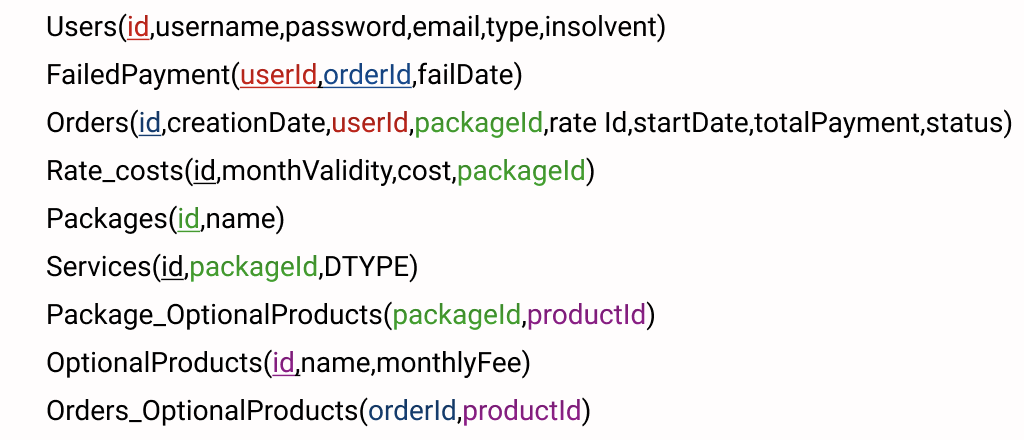
\includegraphics[width=0.80\textwidth]{sqlDDL.png}
\caption{SQL DDL}
\end{figure}
\newpage

Then Services references to three different tables depending on the type of offer:

\begin{figure}[hbt!]
\centering
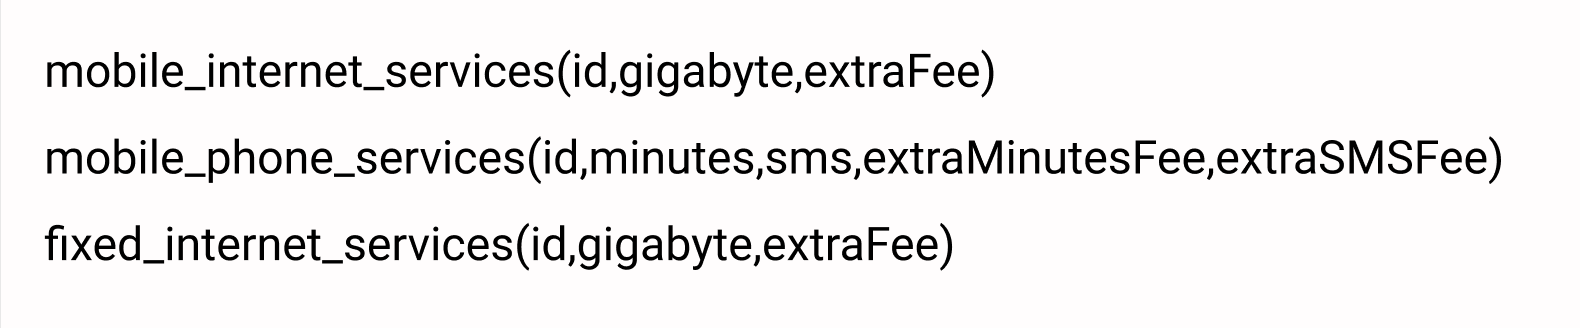
\includegraphics[width=0.70\textwidth]{sqlServicesDDL.png}
\caption{SQL DDL Services Details}
\label{fig:services}
\end{figure}
\subsection{ER Diagram}
In the image can be seen the ER diagram from which we have obtained the tables structure that is shown in next subsection.

\begin{figure}[hbt!]
\centering
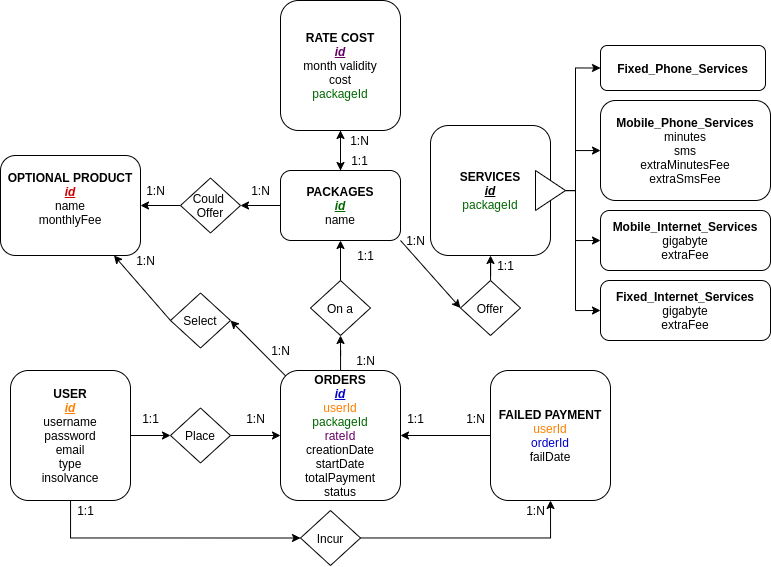
\includegraphics[width=0.99\textwidth]{ER-Simplified.png}
\caption{ER Diagram}
\end{figure}
\subsection{Database visual Schema}
In this section is showed a detailed visualization of the table structure we developed, with all relations, primary and foreign keys.

\begin{figure}[hbt!]
\centering
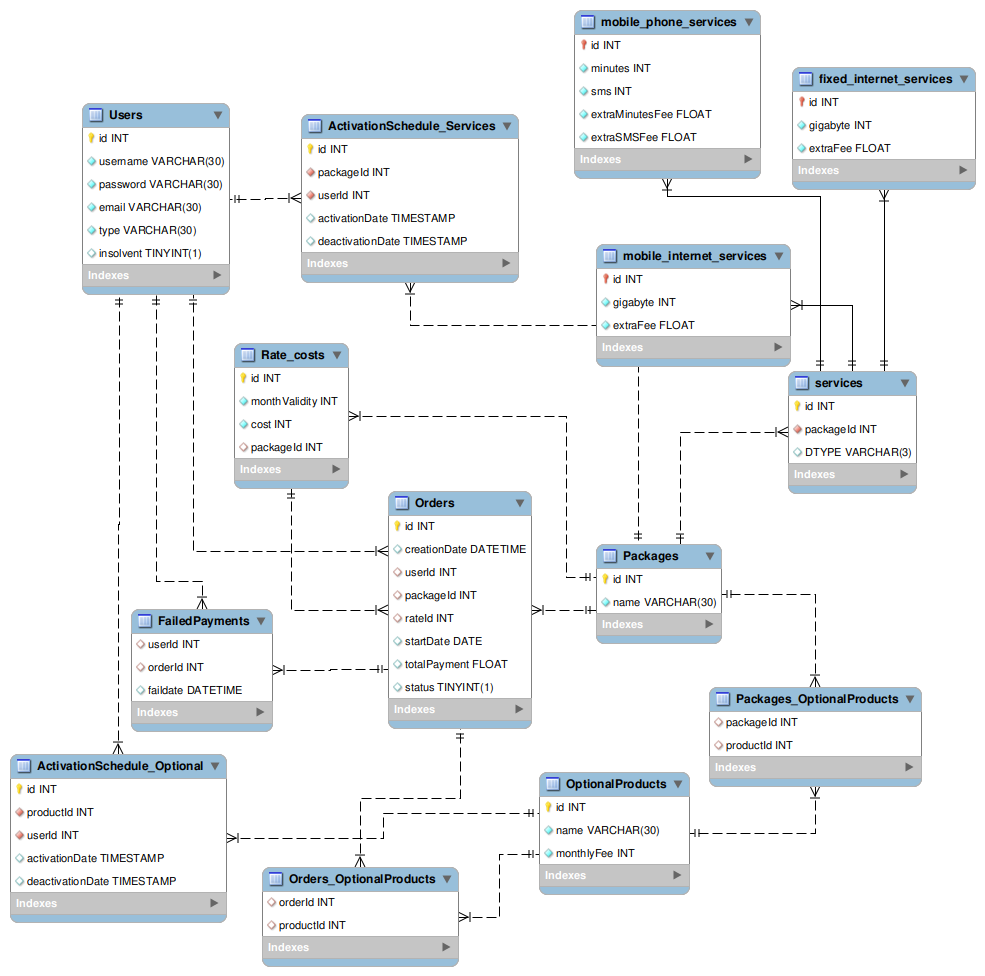
\includegraphics[width=0.99\textwidth]{er2.png}
\caption{ER Diagram}
\end{figure}


\newpage
\section{SQL Description}

Detailed description of SQL code used in the project.
\subsection{Views}
\label{views}
The following views are used for various Sales Reports.
We performed a \emph{selection} for each distinct package (depending on their month validity) and a \emph{count} for their occurrences, Joining Orders and Rate_costs tables.

\begin{lstlisting}
create view PurchasesCount as (
       Select Packages.name as name,Rate_costs.monthValidity as validity, count(*) as count
       from Orders as o join Packages  join Rate_costs
       on o.packageId=Packages.id and Rate_costs.packageId=o.packageId 
       and o.rateId=Rate_costs.id
       group by o.packageId, Rate_costs.id
           );
\end{lstlisting}
Then for a less detailed view, from \emph{PurchasesCount}, a \emph{group by} on the name of the package gives a count of each one.
\begin{lstlisting}
create view PurchasesCountGrouped as (
       select p.name as name, sum(p.count) as count
       from PurchasesCount as p
       group by p.name
           );

\end{lstlisting}

To count the Optional Products was necessary a \emph{left join} because it could exist a Package without any Optional Product, and as a consequence it wouldn't be stored in \emph{Orders_OptionalProducts} table.
\begin{lstlisting}
create view OptionalProductsCount as(
       select o.packageId as packageId, count(opt.productId) as optcount
       from Orders as o left join Orders_OptionalProducts as opt
       on o.id=opt.orderId
       group by o.id
           );
\end{lstlisting}
Then to have the average count of them, we performed an \emph{avg} on the count of previous view.
\begin{lstlisting}
create view OptionalProductsAverage as(
       select p.name as name, avg(opc.optcount) as avg
       from OptionalProductsCount as opc join Packages as p
       where opc.packageId=p.id
       group by id
           );
           
\end{lstlisting}

Following view sums the \emph{totalPayment} of each Order grouped by \emph{packageId}
\begin{lstlisting}
create view ValueOfTotalSales as(
       select p.name as name, sum(o.totalPayment) as totalPayment
       from Orders as o join Packages as p
       where p.id=o.packageId
       group by o.packageId
           );
\end{lstlisting}
Then in \emph{OptionalProductsSales} the same method is used to get the totalCost of the Optional Products related to their corresponding Service Package in \emph{Orderds}
\begin{lstlisting}
create view OptionalProductsSales as(
     select p.name as name,sum(op.monthlyFee*r.monthValidity) as totalOptionalProductsSales
     from Orders_OptionalProducts as orderop join Orders as o
     join OptionalProducts as op join Packages as p join Rate_costs as r
     where o.id=orderop.orderId and orderop.productId=op.id 
     and o.packageId=p.id and o.rateId=r.id
     group by p.id
          );
\end{lstlisting}

And finally these two views are \emph{left joined} to have both \emph{totalPayment} with and without Optional Products. A \emph{left join} is required because as mentioned before it could exist a service package without Optional Product. In this case \emph{totalPaymentWithoutOP} will return \emph{null}.
\begin{lstlisting}
create view ValueOfSalesDetailed as(
       select vot.name as name, vot.totalPayment as totalPayment, 
               (vot.totalPayment-ops.totalOptionalProductsSales) as totalPaymentWithoutOP
       from ValueOfTotalSales as vot left join OptionalProductsSales as ops
       on vot.name=ops.name
         );
\end{lstlisting}                                     


In \emph{InsolventReport} are selected all Users with \emph{having count(*)>=3} of insolvent orders stored in \emph{FailedPayments}.
\begin{lstlisting}
create view InsolventReport as(
        select u.id as id,u.username as username,u.email as email,
              (
              select max(fp1.faildate) 
              from FailedPayments as fp1  
              where fp1.userId=u.id) as lastDate,
              (
              select o.totalPayment 
              from Orders as o join FailedPayments as fp2 
              where o.id=fp2.orderId and lastdate=fp2.faildate) as amount
        from FailedPayments as fp join Users as u
        where fp.userId=u.id
        group by u.id
        having count(*)>=3
           );
\end{lstlisting}

Last view  \emph{OptionalProductBestSeller} is used to have a count and the value of total sales of each Optional Product.
\begin{lstlisting}
create view OptionalProductBestSeller as(
        select op.name as name,count(op.id) as amountSold, 
               sum(op.monthlyFee*r.monthValidity) as value
        from Orders_OptionalProducts as ordop join OptionalProducts as op 
        join Rate_costs as r join Orders as o
        where ordop.productId=op.id and o.rateId=r.id and o.id=ordop.orderId
        group by op.id
             );
\end{lstlisting}
The using two distinct queries we performed the  \emph{OptionalProductBestSellerForValue}
\begin{lstlisting}
        select o 
        from OptionalProductBestSeller o 
        where o.value=(
        select max(o2.value) 
        from OptionalProductBestSeller o2
        );
\end{lstlisting}
and  \emph{OptionalProductBestSellerForAmount}
\begin{lstlisting}
          select o from OptionalProductBestSeller o 
          where o.amountSold=(
          select max(o2.amountSold) 
          from OptionalProductBestSeller o2
          );
\end{lstlisting}
\newpage
\subsection{Triggers}
\subparagraph{INSOLVENT_USER}
When a new order is created, if it's status is "false" then mark user as insolvent by changing a boolean into user table.
\begin{lstlisting}
create trigger INSOLVENT_USER
    after insert on Orders
    for each row
	begin
		if ( new.status = false) then
		update Users set Users.insolvent = true where Users.id = new.userId;
		insert into FailedPayments (userId,orderId,faildate) 
		values (new.userId,new.id,CURRENT_TIMESTAMP);
	end if;
	END $$
\end{lstlisting}
\subparagraph{INSOLVENT_USER_REMOVAL}
When an order is updated, if it's status is "true" then remove insolvance status from user.

\begin{lstlisting}
create trigger INSOLVENT_USER_REMOVAL
    after update on Orders
    for each row
	begin
	-- user payed a suspended order i check if all his pending order are payed (if yes remove flag)
		if (new.status = true) AND (select count(*) from Orders as o 
								   where o.userId=new.userId and o.status = false) = 0
			then
		update Users set Users.insolvent = false where Users.id = new.userId;
	end if;
	if (new.status = false AND old.status = new.status)  then
				insert into FailedPayments (userId,orderId,faildate) 
				values (new.userId,new.id,CURRENT_TIMESTAMP);
	end if;
	END $$
\end{lstlisting}

\subparagraph{NewPackage}
When a new package is created some view are initialized with a new row containing the package name and empty values for the statistic field (eg: AVG,totalPayments...)
\begin{lstlisting}
    create trigger NewPackage
		after insert on Packages
        for each row
        begin
			-- Optional Average per package
			insert into OptionalProductsAverage (name,avg) values (new.name ,0);
            -- Revenue per package
            insert into ValueOfSalesDetailed  (name,totalPayment,totalPaymentWithoutOP) 
            values (new.name,0,0);
        END $$
\end{lstlisting}

\subparagraph{PurchaseCountInitialize}
When a new package is created are created also the rate cost, so as in the  "NewPackage" trigger and for each new RateCost a new row with initial value is added to "PurchaseCount" view
\begin{lstlisting}
create trigger PurchaseCountInitialize 
		after insert on Rate_costs
        for each row
        begin
			declare pkgname Varchar(30);
			set pkgname   := (select name from Packages where Packages.id=new.packageId);
			insert into PurchasesCount (name,validity,count) 
			values (pkgname,new.monthValidity,0);
        END$$
\end{lstlisting}

\subparagraph{PurchasesCount_Population}
Whenever an Order is created and has a valid payment this table increase the number of time the package is payed
\begin{lstlisting}
create trigger PurchasesCount_Population
	after insert on Orders 
    for each row
	begin
	declare pkgname Varchar(30);
    declare orderVal int;
    if new.status = true then
    set pkgname   := (select name from Packages where Packages.id=new.packageId);
    set orderVal  := (select monthValidity from Rate_costs where id=new.rateId);
		 -- If this is the first order on package then set count = 1 and insert new line
            SET SQL_SAFE_UPDATES=0;
			update PurchasesCount set PurchasesCount.count = PurchasesCount.count + 1
					where name = pkgname and validity = orderVal;
            SET SQL_SAFE_UPDATES=1;
        end if;
	END $$
\end{lstlisting}

\subparagraph{PurchasesCount_Population_Update}
Same as PurchasesCount_Population but when Order is updated, check if payment is ok then update view.
\begin{lstlisting}
create trigger  PurchasesCount_Population_Update
    after update on Orders
    for each row
	begin
	declare pkgname Varchar(30);
    declare orderVal int;
    if new.status = true then
		set pkgname   := (select name from Packages where Packages.id=new.packageId);
		set orderVal  := (select monthValidity from Rate_costs where id=new.rateId);

            SET SQL_SAFE_UPDATES=0;
			update PurchasesCount set PurchasesCount.count = PurchasesCount.count + 1
					where name = pkgname and validity = orderVal;
            SET SQL_SAFE_UPDATES=1;
        end if;
    END $$
\end{lstlisting}

\subparagraph{AddNoOptionalOrderToAVG}
This trigger is a "support trigger" because is used to call another trigger.
When an order is created add a "fake null optionalProduct" to it so that Order with no product are counted in the Average.(See next trigger)
\begin{lstlisting}
create trigger AddNoOptionalOrderToAVG
	after insert on Orders
    for each row
    begin
		-- trigger OptionalProdAvg trigger
		insert into Orders_OptionalProducts (orderId,productId) values (new.id,null);
		delete from Orders_OptionalProducts where orderId = new.id;
    END $$
\end{lstlisting}

\subparagraph{OptionalProdAvg}
When a new product is associated to a new order, after checking if payment is ok update the average of the specific product that is been added.
\begin{lstlisting}
create trigger OptionalProdAvg
	after insert on Orders_OptionalProducts
	for each row
    begin
    declare pkgcount INT;
    declare pkgname Varchar(30);
    declare stat  bool;
    set stat    := (select status from Orders where id=new.orderId);
    if stat = 1 then
    set pkgname   := (select name from Packages 
    where Packages.id=(select packageId from Orders where id=new.orderId));
	set pkgcount  := (select count(*) from PurchasesCountGrouped 
	group by name having name = pkgname) - 1;
	SET SQL_SAFE_UPDATES=0;
    if(new.productId is null) then
		update OptionalProductsAverage 
		set avg = ((avg*pkgcount))/(pkgcount+1) where name=pkgname;
    else 
		update OptionalProductsAverage 
		set avg = ((avg*pkgcount)+1)/(pkgcount+1) where name=pkgname;
    end if;
    SET SQL_SAFE_UPDATES=1;
        end if;
    END $$
\end{lstlisting}

\subparagraph{OptionalProdAvgOnUpdate}
When an order is updated, if payment is ok, this trigger calculate how many optional is associated with it and update the AVG of the package in consequence.
\begin{lstlisting}
create trigger OptionalProdAvgOnUpdate
	after update on Orders
    for each row
    begin
	declare pkgcount INT;
    declare pkgname Varchar(30);
    declare prodCount INT;
    if new.status then
    set pkgname   := (select name from Packages 
    			where Packages.id=(select packageId from Orders where id=new.id));
	set pkgcount  := (select count(*) from PurchasesCountGrouped 
			group by name having name = pkgname);
    set prodCount := (select count(*) from Orders_OptionalProducts 
    			group by orderId having  orderId= new.id) -1;
			SET SQL_SAFE_UPDATES=0;
            if(prodCount is null) then
				update OptionalProductsAverage 
				set avg = ((avg*pkgcount))/(pkgcount+1) where name=pkgname;
            else 
				update OptionalProductsAverage 
				set avg = ((avg*pkgcount)+prodCount)/(pkgcount+1) where name=pkgname;
            end if;
            SET SQL_SAFE_UPDATES=1;
        end if;
    END $$
\end{lstlisting}

\subparagraph{TotalPackageRevenue}
When a new order is created, if payment is ok update this view with totalRevenue of this package 
(see trigger PackageRevenueNoOptional to see how the OptionalRevenue is removed from totalRevenue).
\begin{lstlisting}
create trigger TotalPackageRevenue
	after insert on Orders
    for each row
    begin
    declare pkgname Varchar(20);
    declare validity int;
	declare totalOfProducts int;
    if new.status = 1 then
		set pkgname   := (select name from Packages where Packages.id=new.packageId);
		set validity  := (select monthValidity from Rate_costs where id=new.rateId);
			SET SQL_SAFE_UPDATES=0;
				update ValueOfSalesDetailed 
				set totalPayment =  totalPayment + new.totalPayment ,
                     totalPaymentWithoutOP = totalPaymentWithoutOP + new.totalPayment
				where name=pkgname;
			SET SQL_SAFE_UPDATES=1;                     
        end if;
    END $$
\end{lstlisting}

\subparagraph{PackageRevenueNoOptional}
For each product associated with order it query the revenue of it and remove it from the total revenue of the package.
\begin{lstlisting}
-- remove optional revenue for each optional
create trigger PackageRevenueNoOptional 
	after insert on Orders_OptionalProducts
    for each row
    begin
    declare pkgId     INT;
	declare pkgname Varchar(20);
	declare price     INT;
    declare validity  INT;
	declare stat  bool;
    set stat    := (select status from Orders where id=new.orderId);

    if stat = 1 then
		 
         set pkgId     := (select packageId from Orders where id=new.orderId);
		 set pkgname   := (select name from Packages where Packages.id=pkgId);
         set validity  := (select monthValidity from Rate_costs 
         				  where id=(select rateId from Orders where id=new.orderId));
		 set price     := (select monthlyFee from OptionalProducts 
		 				where id=new.productId)*validity;
         
         if(price is null)then
			set price := 0;
         end if;
        SET SQL_SAFE_UPDATES=0;    
        update ValueOfSalesDetailed set 
				totalPaymentWithoutOP = totalPaymentWithoutOP - price
				where name=pkgname;
		SET SQL_SAFE_UPDATES=1; 
        
	end if;
    END $$
\end{lstlisting}

\subparagraph{TotalPackageRevenue_Update}
When Order is updated, check if payment is ok and as before it calculate optional prod revenue and remove it from the totalRevenue of this package.
\begin{lstlisting}
create trigger TotalPackageRevenue_Update
	after update on Orders
	for each row
    begin
    declare pkgname Varchar(30);
	declare revenueOptional   INT;
    declare validity  INT;
		if new.status = 1 then
			set pkgname   := (select name from Packages where Packages.id=new.packageId);
			set validity  := (select monthValidity from Rate_costs 
				where id=(select rateId from Orders where id=new.id));
				set revenueOptional := (select sum(monthlyFee) 
				from Orders_OptionalProducts join OptionalProducts on productId = id 
				group by orderId having orderId=new.id)*validity;
        
			if(revenueOptional is null) then
				set revenueOptional := 0;
			end if;
        
			SET SQL_SAFE_UPDATES=0;
				update ValueOfSalesDetailed 
				set totalPayment =  totalPayment + new.totalPayment ,
                		totalPaymentWithoutOP = totalPaymentWithoutOP + (new.totalPayment -revenueOptional)
					where name=pkgname;
			SET SQL_SAFE_UPDATES=1;                     
        end if;
    END$$
\end{lstlisting}

\subparagraph{InitializeBestOptional}
Initialize the BestOptional view whenever a new optional product occur
\begin{lstlisting}
create trigger InitializeBestOptional
	after insert on OptionalProducts
    for each row
    begin
		insert into OptionalProductBestSeller (name,amountSold,value) values (new.name,0,0);
    END$$
\end{lstlisting}

\subparagraph{UpdateBestOptional}
Whenever a product is associated with an order this trigger update the view that contain statistic about best optional.
It calculate the revenue for this new product and sum it to the total revenue of it
It increase the counter of how many time this product have been bought.
\begin{lstlisting}
    
create trigger UpdateBestOptional
    after insert on Orders_OptionalProducts
	for each row
    begin
		 declare prodName Varchar(30);
         declare price     INT;
         declare validity  INT;
         
         declare stat  bool;
		set stat    := (select status from Orders where id=new.orderId);

		if stat = 1 then
		 set prodName  := (select name from OptionalProducts where id=new.productId);
         set validity  := (select monthValidity from Rate_costs 
         		where id=(select rateId from Orders where id=new.orderId));
		 set price     := (select monthlyFee from OptionalProducts 
		 		where id=new.productId)*validity;
         
			if(prodName is not null) then
			 SET SQL_SAFE_UPDATES=0;    
				update OptionalProductBestSeller set value = value + price,
													 amountSold = amountSold + 1 
													 where name=prodName;
				SET SQL_SAFE_UPDATES=1;    
			 end if;
        end if;
    END$$
\end{lstlisting}

\subparagraph{UpdateBestOptional_OnUpdate}
Same as UpdateBestOptional but with a unique query for all product associated with this order (more expensive but only way if the first payment fail)
\begin{lstlisting}
    create trigger UpdateBestOptional_OnUpdate
	after update on Orders
    for each row
		begin
         declare revenue     INT;
         declare validity  INT;
		 declare count  INT;
		 set validity  := (select monthValidity from Rate_costs where id=(select rateId from Orders where id=new.id));
		if new.status = 1 then
			 SET SQL_SAFE_UPDATES=0;    
				update OptionalProductBestSeller as best join OptionalProducts as op
									on best.name = op.name
									set amountSold = amountSold + 1,
									value = value + op.monthlyFee * validity
									where op.name in (select op1.name from OptionalProducts as op1 join Orders_OptionalProducts as ord
													on id = productId where ord.orderId =new.id);
				SET SQL_SAFE_UPDATES=1;    
		end if;
	END $$
\end{lstlisting}

\subparagraph{UpdateInsolventUser}
When a user fail a payment this trigger count how many time is happened and if it happen more then 3 times it update (or insert) a line with the last failed payment (date,amount).
\begin{lstlisting}

create trigger UpdateInsolventUser
    after insert on FailedPayments
	for each row
    begin
		declare failedCount INT;
        declare failedImport INT;
        declare usr Varchar(30);
        declare mail	 Varchar(30);

        set failedCount := (select count(*) from FailedPayments  group by userId having userId = new.userId );
        set failedImport := (select totalPayment from Orders where id=new.orderId);
        set usr := (select username from Users where id=new.userId);
        set mail    := (select email from Users where id=new.userId);
        
         -- SIGNAL SQLSTATE '02000' SET MESSAGE_TEXT =username ;
        if(failedCount >=3) then
			if( (select id from InsolventReport where id=new.userId) is  null) then
				insert into InsolventReport (id,username,email,lastDate,amount) values (new.userId,usr ,mail ,new.faildate,failedImport);
			else
				update InsolventReport set lastDate = new.faildate, amount = failedImport where id=new.userId;
			end if;
        end if;
    END$$
\end{lstlisting}
\newpage

\section{ORM Description}

\subsection{Entities}
\lstset{language=Java}
\paragraph{Optional Product}
Entity related to all type of optional products with id and related name.
\begin{lstlisting}
@Entity
@Table(name = "OptionalProducts", schema = "test")
public class OptionalProduct{

    @Id
    @GeneratedValue(strategy= GenerationType.IDENTITY)
    int     id;
    String  name;
    int     monthlyFee;
\end{lstlisting}

\paragraph{Order}
The Order entity refers to Table \emph{Orders}, with a boolean \emph{status} that is true if the payment has been accepted from bank. The \emph{bank} pseudo application works at follows: the first payment is completely pseudo-random (using \emph{Random} java library). Then if the order is insolvent the purchase process is always accepted for demo purposes.
\begin{lstlisting}
@Entity
@Table(name = "Orders", schema = "test")
@NamedQuery(name="Orders.Id" ,  query="select o from Order o where o.Id = :orderId")
@NamedQuery(name="Orders.All" , query="select o from Order o") @NamedQuery(name="Orders.Suspended" , query="select o from Order o where o.status=false")
@NamedQuery(name="Orders.RemoveSuspend" , query="update Order o set o.status = true where o.Id=:orderId")
@NamedQuery(name="PurchasesByPackages" , query = "select count (distinct o) from Order o group by o.pack")
@NamedQuery(name="PurchasesByPackagesID" , query = "select  o.pack.name, count(o.pack) from Order o where o.status=true group by o.pack ")
@NamedQuery(name="Orders.UserInsolvances" , query = "select o from Order o where o.status=false and o.user.id = :userId")

public class Order {

    @Id
    @GeneratedValue(strategy= GenerationType.IDENTITY)
    int Id;
    Date startDate;
    Date creationDate;
    float totalPayment;
    Boolean status =null;
    
\end{lstlisting}


\paragraph{RateCost}
Entity of a package rate cost, depending on the \emph{monthValidity} period.
\begin{lstlisting}
@Entity
@Table(name="Rate_costs", schema = "test")
public class RateCost {

    @Id
    @GeneratedValue(strategy= GenerationType.IDENTITY)
    int id;
    int monthValidity;
    int cost;
    @ManyToOne(fetch = FetchType.LAZY)
    @JoinColumn(name = "packageId")
\end{lstlisting}

\paragraph{Service}
Entity of services, used as a connection between \emph{Packages} and various services as mentioned in figure \ref{fig:services}
\begin{lstlisting}
@Entity
@Inheritance(strategy = InheritanceType.JOINED)
@Table(name = "services", schema = "test")
public class Service {
    @Id
    @GeneratedValue(strategy=GenerationType.IDENTITY)
    int id;
    @ManyToOne(fetch = FetchType.LAZY)
    @JoinColumn(name = "packageId")
    Package packageId;
    @Column(name = "DTYPE")
    String type;
\end{lstlisting}

\paragraph{User}
Entity with data of users, and boolean \emph{Insolvent} to determine if there are three or more purchases not completed.
\begin{lstlisting}
@Entity
@NamedQuery(name = "User.authentication", query = "select usr from User usr WHERE usr.username = :username and usr.password = :password")
@NamedQuery(name = "User.insolvent"     , query = "select usr from User usr WHERE usr.insolvent = true")
@Table(name="Users", schema = "test")
public class User {
    @Id
    @GeneratedValue(strategy=GenerationType.IDENTITY)
    int id;

    String  username;
    String  password;
    String  email;
    String  type;
    boolean insolvent;
\end{lstlisting}

\paragraph{Package}
Entity of purchased packages with its rates, services and optional products.
\begin{lstlisting}
@Entity
@NamedQuery(name="Packages.All",query="select p from Package p")
@Table(name = "Packages", schema = "test")
public class Package {
    @Id
    @GeneratedValue(strategy=GenerationType.IDENTITY)
    int     id;
    String  name;


    @OneToMany(cascade=CascadeType.PERSIST)
    @JoinColumn(name = "packageId")
    List<Service> services;

    @OneToMany(cascade=CascadeType.PERSIST)
    @JoinColumn(name = "packageId")
    List<RateCost> rates;

    @JoinTable(
            name = "Packages_OptionalProducts",
            schema = "test",
            joinColumns = @JoinColumn(name = "packageId"),
            inverseJoinColumns = @JoinColumn(name = "productId"))
    @ManyToMany(cascade=CascadeType.PERSIST)
    List<OptionalProduct> products;
\end{lstlisting}

\paragraph{Custom}
Furthermore to manage the views, some custom classes have been created to store query views correctly. These classes reflect exactly the type of data queried in Views from page \pageref{views}.
A list of them:
\begin{itemize}
    \item InsolventReport
    \item OptionalProductBestSeller
    \item OptionalProductsAverage
    \item PurchasesCoun
    \item PurchasesCountGrouped
    \item ValueOfSalesDetailed
\end{itemize}

\newpage
\section{Application Components}
\subsubsection{Services:}
\begin{figure}[hbt!]
\centering
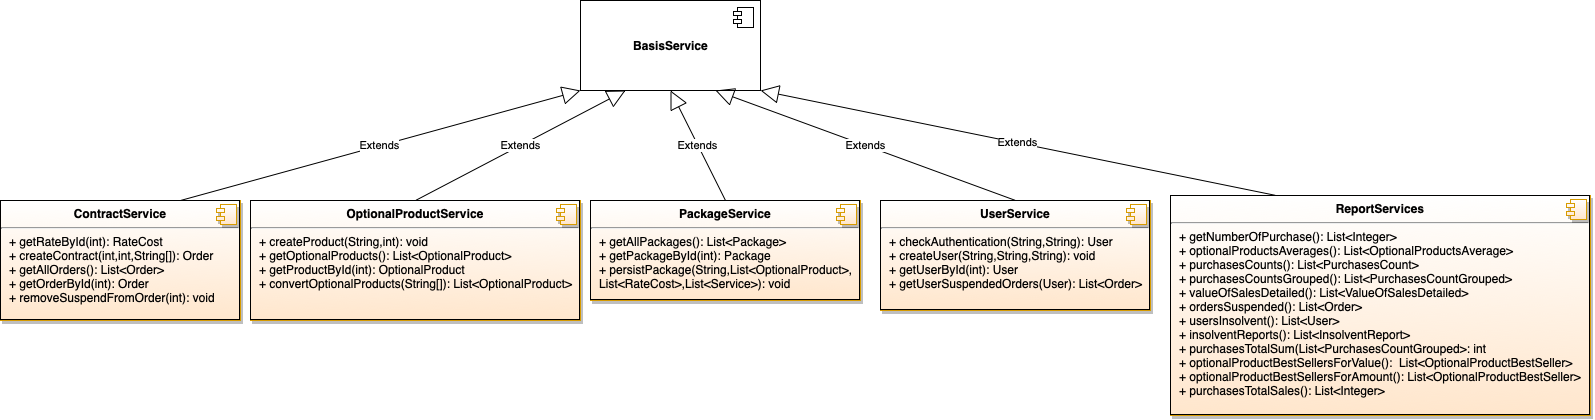
\includegraphics[width=0.99\textwidth]{services.png}
\caption{Services}
\end{figure}
\subsubsection{Controllers:}
\begin{figure}[hbt!]
\centering
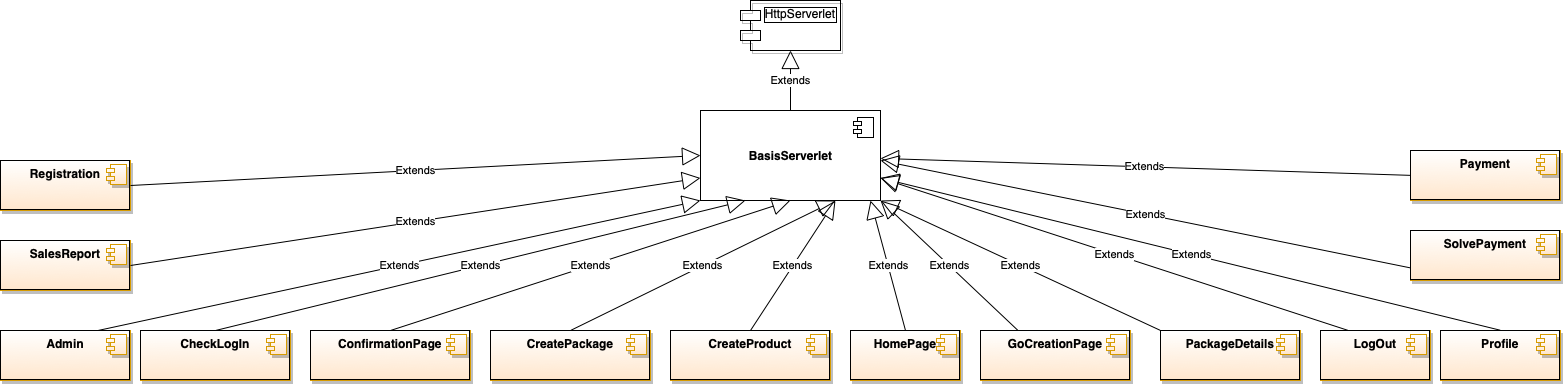
\includegraphics[width=0.99\textwidth]{controllers.png}
\caption{Controllers}
\end{figure}
\begin{itemize}
	\item \textbf{checkLogin} to manage login operation
	\item \textbf{Registreation} to manage registration operation
	\item \textbf{HomePage} to redirect user to the homepage and render all the packages available
	\item \textbf{PackageDetails} to display details of a specific package
	\item \textbf{ConfirmationPage} to display all date of the contract chosen by user
	\item \textbf{Payment} to simulate payment system
	\item \textbf{GoCreatePackage} to allow admin package creation
	\item \textbf{GoCreateProduct} to allow admin optional product creation
\end{itemize}

\newpage
\section{UML sequence diagrams}

\begin{figure}[hbt!]
\centering
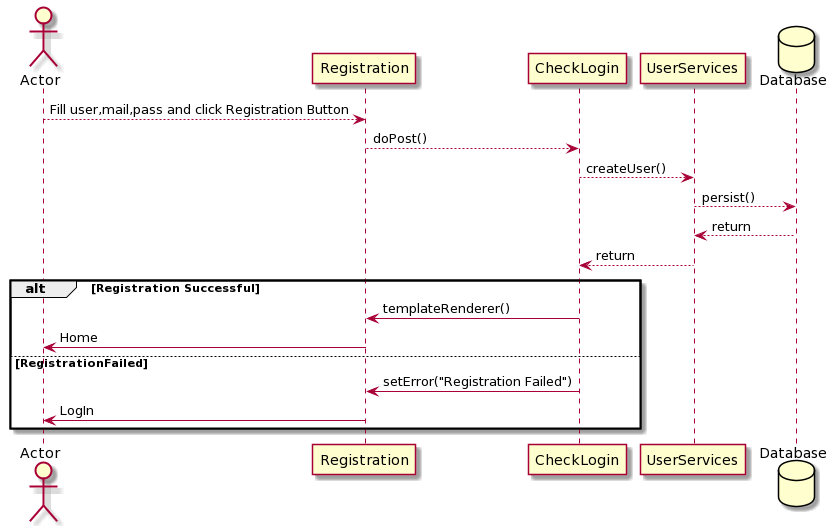
\includegraphics[width=0.99\textwidth]{Registration.png}
\caption{Registration}
\end{figure}

\begin{figure}[hbt!]
\centering
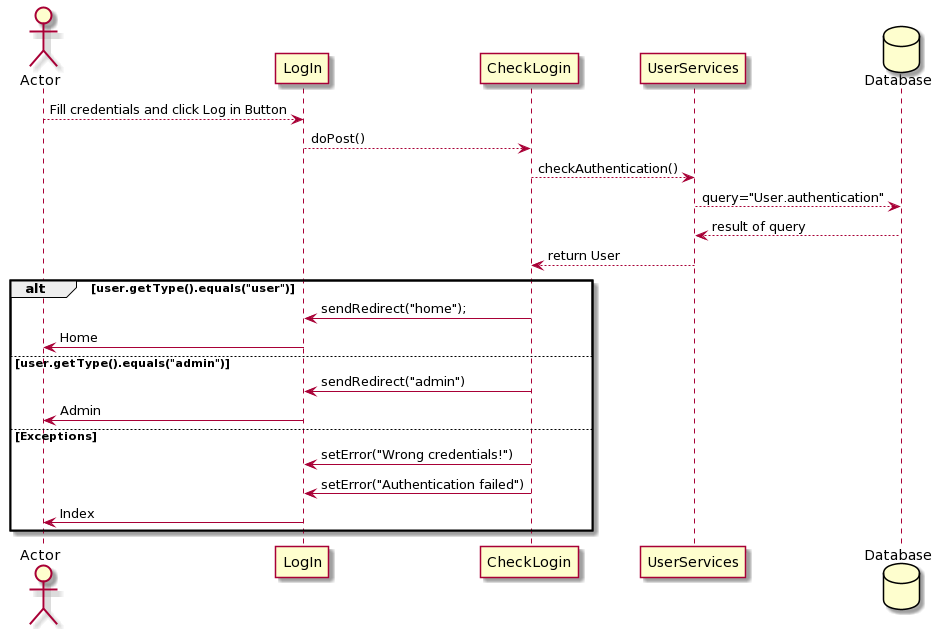
\includegraphics[width=0.99\textwidth]{LogIn.png}
\caption{Log In}
\end{figure}

\begin{figure}[hbt!]
\centering
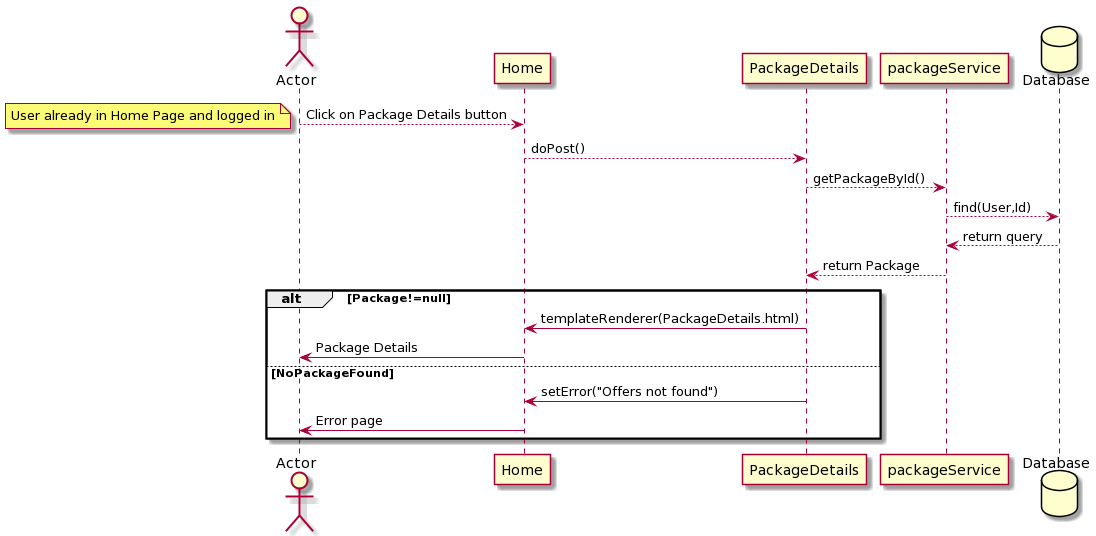
\includegraphics[width=0.99\textwidth]{PackDetails.png}
\caption{Package Details}
\end{figure}

\begin{figure}[hbt!]
\centering
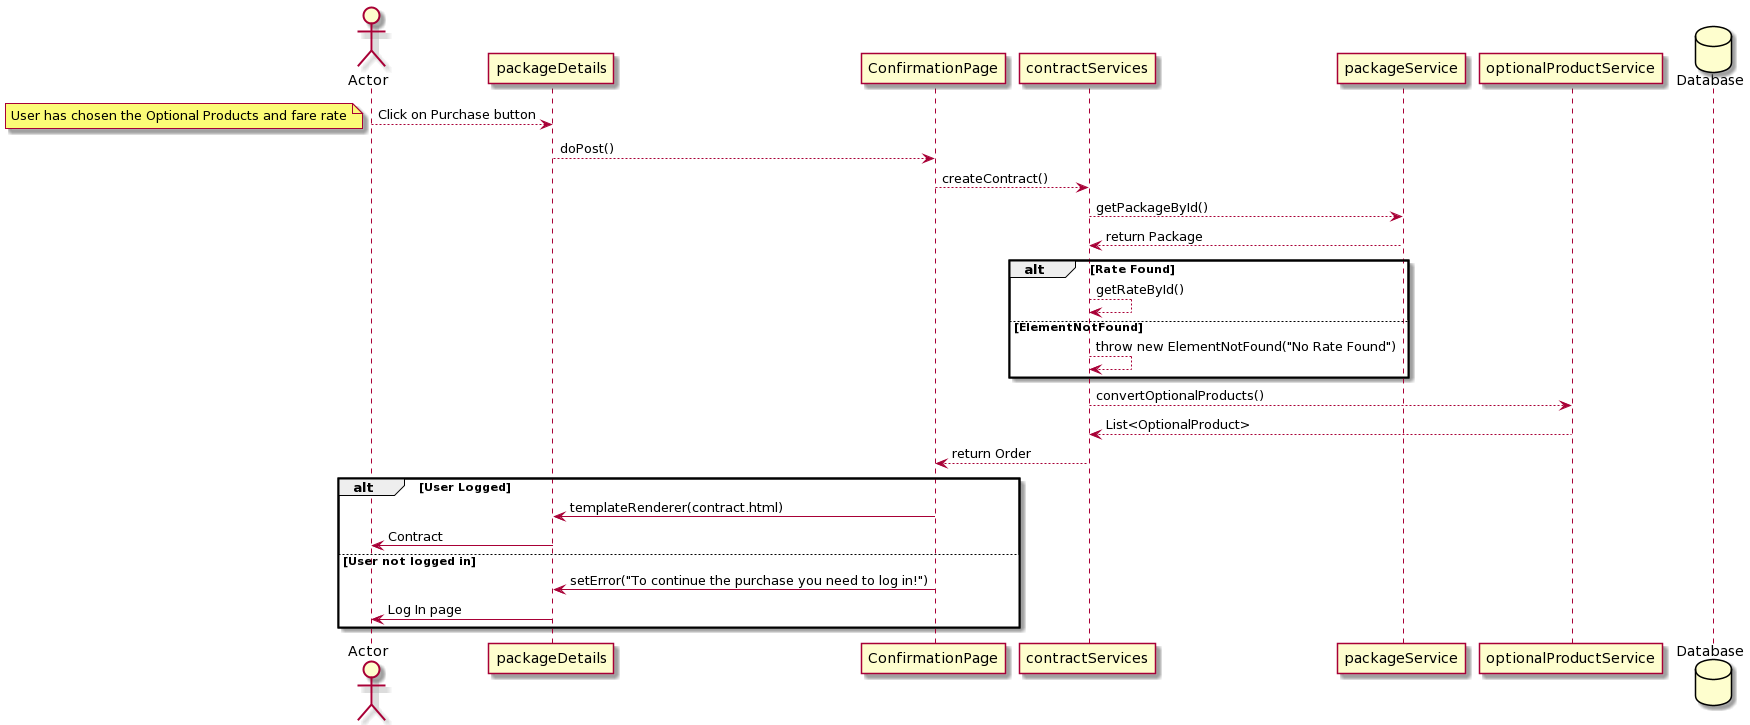
\includegraphics[width=0.99\textwidth]{Buy.png}
\caption{Purchase}
\end{figure}


\begin{figure}[hbt!]
\centering
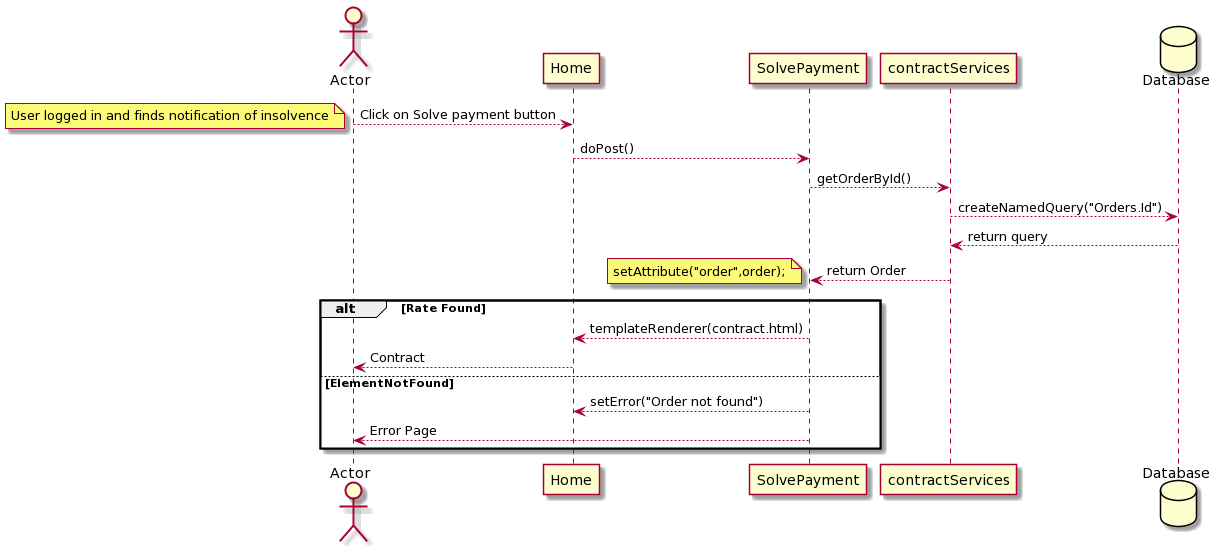
\includegraphics[width=0.99\textwidth]{Insolvent.png}
\caption{Insolvent User}
\end{figure}

\begin{figure}[hbt!]
\centering
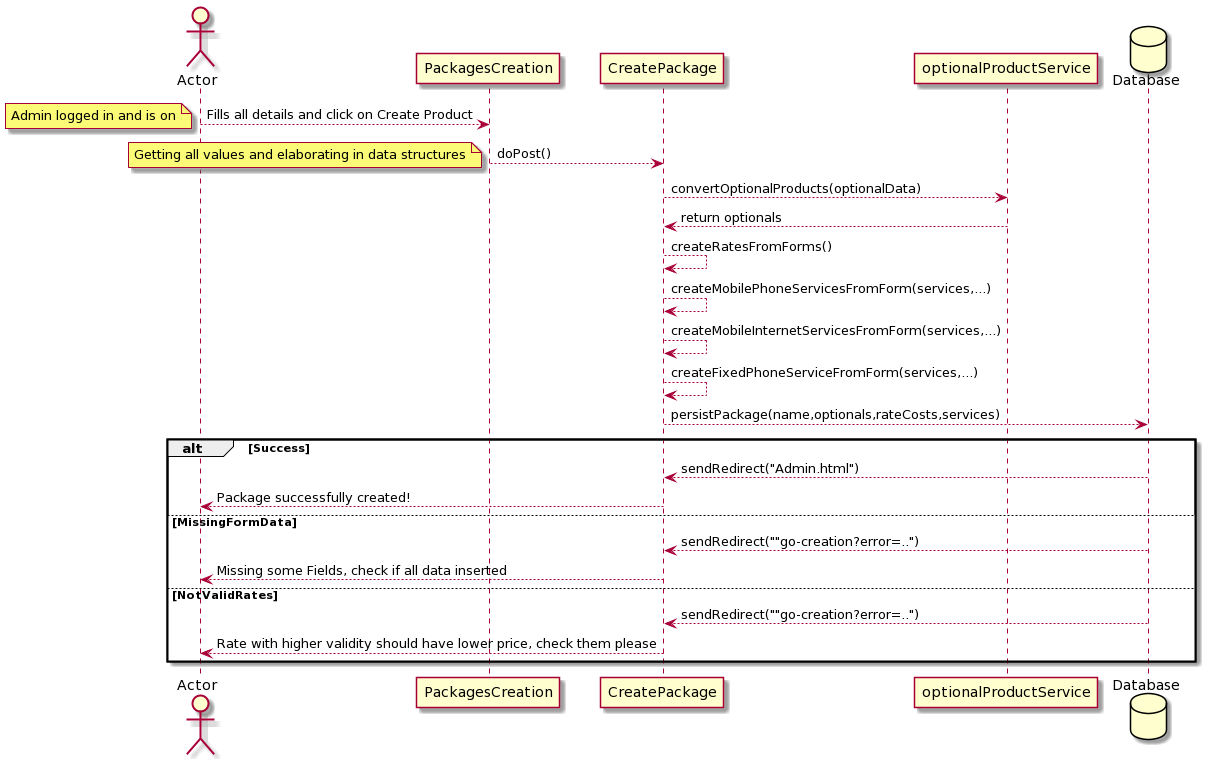
\includegraphics[width=0.99\textwidth]{Creation.png}
\caption{Package Creation}
\end{figure}
\end{document}